% ============================================================
% Chapter 4 — Experimental Evaluation
% ============================================================
\chapter{Experimental Evaluation}
\label{ch:results}

This chapter presents the experimental evaluation of AnyUp3D.
Section~\ref{sec:setup} describes the experimental setup, including hardware, backbone, model configuration, and training details.
Section~\ref{sec:convergence} provides a qualitative analysis of training convergence by comparing early and late checkpoints.
Section~\ref{sec:temporal} evaluates temporal feature consistency against the frame-independent 2D~AnyUp baseline across the full DAVIS~2017 validation set.
Section~\ref{sec:jf} measures the downstream impact of AnyUp3D features on video object segmentation using the standard $\mathcal{J}\&\mathcal{F}$ metric.
Finally, Section~\ref{sec:discussion} discusses the results, identifies failure cases, and acknowledges limitations.


% ────────────────────────────────────────────
\section{Experimental Setup}
\label{sec:setup}

% ── 4.1.1 Hardware & Software ──
\subsection{Hardware and Software}

All experiments were conducted on Google Colab using a single NVIDIA T4 GPU with 16\,GB of video memory.
The implementation uses PyTorch 2.x with CUDA, and all models were run in mixed-precision (\texttt{float16}) where supported to fit within the T4's memory budget.

% ── 4.1.2 Backbone ──
\subsection{Backbone}

We use VideoMAE~\cite{videomae} (ViT-B/16, pretrained on Kinetics-400~\cite{kay2017kinetics}) as the spatiotemporal feature extractor throughout all experiments.
VideoMAE processes 16 input frames using a tubelet size of~2, producing $T' = 8$ temporal tokens.
Each frame is patchified at $16 \times 16$, yielding a spatial resolution of $14 \times 14$ per temporal slice.
The resulting feature tensor has shape $(1, 768, 8, 14, 14)$ — that is, 768-dimensional features at $8 \times 14 \times 14$ spatiotemporal positions.

We chose VideoMAE because it produces genuinely spatiotemporal tokens: its tubelet embedding jointly encodes pairs of adjacent frames, so the features at each position already carry short-range temporal context.
This makes it a natural input for AnyUp3D, which extends this temporal structure to the upsampled resolution.

% ── 4.1.3 AnyUp3D Configuration ──
\subsection{AnyUp3D Configuration}

The AnyUp3D model is configured with a query/key dimension of $d_{qk} = 128$, four attention heads, a spatial kernel size of~1, and a window ratio of~0.1.
The temporal kernel size in the 3D convolutions is set to $t_k = 3$.
These hyperparameters match the 2D~AnyUp defaults where applicable, with the temporal kernel size chosen to allow each feature position to attend to its immediate temporal neighbors.

% ── 4.1.4 Training ──
\subsection{Training Details}

AnyUp3D was trained for 6{,}000 steps using the AdamW optimizer with a learning rate of $2 \times 10^{-4}$.
Training followed the T-curriculum strategy described in Chapter~3: beginning with $T\!=\!2$ frames to warm up the spatial upsampling pathway, then increasing to $T\!=\!4$ at step 5{,}000.
The third stage ($T\!=\!8$, scheduled to activate at step 15{,}000) was never reached, as training concluded at step 6{,}000; in practice, only the $T\!=\!2$ and $T\!=\!4$ stages were completed.
The objective function combines four loss terms: $\mathcal{L}_\text{cos-mse}$, $\mathcal{L}_\text{input-consistency}$, $\mathcal{L}_\text{self-consistency}$, and $\mathcal{L}_\text{temporal-consistency}$ with RGB-difference gating, as detailed in Section~\ref{sec:losses} of Chapter~3.

% ── 4.1.5 Evaluation Dataset ──
\subsection{Evaluation Dataset}

All evaluations use the DAVIS~2017 validation set~\cite{davis2017}, a standard video object segmentation benchmark containing 30 video clips with pixel-level ground-truth annotations.
DAVIS~2017 is well suited for this evaluation: its clips are short enough to process on a T4 GPU, cover diverse motion types (from slow camera pans to fast athletic movements), and provide ground-truth masks that enable both quantitative and qualitative assessment.

% ── 4.1.6 Baselines ──
\subsection{Baselines}

We compare AnyUp3D against two baselines:

\paragraph{Bilinear upsampling.}
The VideoMAE feature tensor at $14 \times 14$ spatial resolution is upsampled to $224 \times 224$ using trilinear interpolation, independently per channel.
This baseline requires no learned parameters and represents the simplest possible spatial upsampling strategy.

\paragraph{2D AnyUp (frame-independent).}
The pretrained 2D~AnyUp model~\cite{anyup} is applied independently to each frame.
Each temporal slice of the VideoMAE feature tensor is treated as a separate image-level feature map and upsampled using the original AnyUp architecture with no temporal context.
This baseline isolates the contribution of the temporal extension: any improvement of AnyUp3D over this baseline is attributable to the 3D temporal modeling rather than the spatial cross-attention mechanism, which both models share.


% ────────────────────────────────────────────
\section{Experiment 1: Training Convergence}
\label{sec:convergence}

Before evaluating AnyUp3D on benchmark metrics, we verify that the model learns meaningful spatial structure during training.
We do so by comparing the upsampled features produced by an early checkpoint (step~250) against the final checkpoint (step~6{,}000), applied to the same input video.

\subsection{Setup}

A short video clip is processed through VideoMAE to produce features of shape $(1, 768, 8, 14, 14)$.
Both checkpoints receive the same low-resolution features and the same RGB guide video, and produce upsampled output at $224 \times 224$ spatial resolution.
We visualize the output using PCA: the top three principal components of the 768-dimensional feature vectors are mapped to RGB channels, with PCA fitted jointly across all frames to ensure color consistency over time.

\subsection{Results}

% ── FIGURE: Step 250 vs Step 6000 PCA ──
\begin{figure}[t]
    \centering
    % [Figure 1: Side-by-side PCA visualization.
    %  Row 1: Original video frames (8 frames, t=0 to t=7).
    %  Row 2: PCA of AnyUp3D output at step 250 — features appear
    %          noisy and spatially unstructured.
    %  Row 3: PCA of AnyUp3D output at step 6000 — features show
    %          clear object boundaries and spatially coherent regions
    %          that track the objects across frames.]
    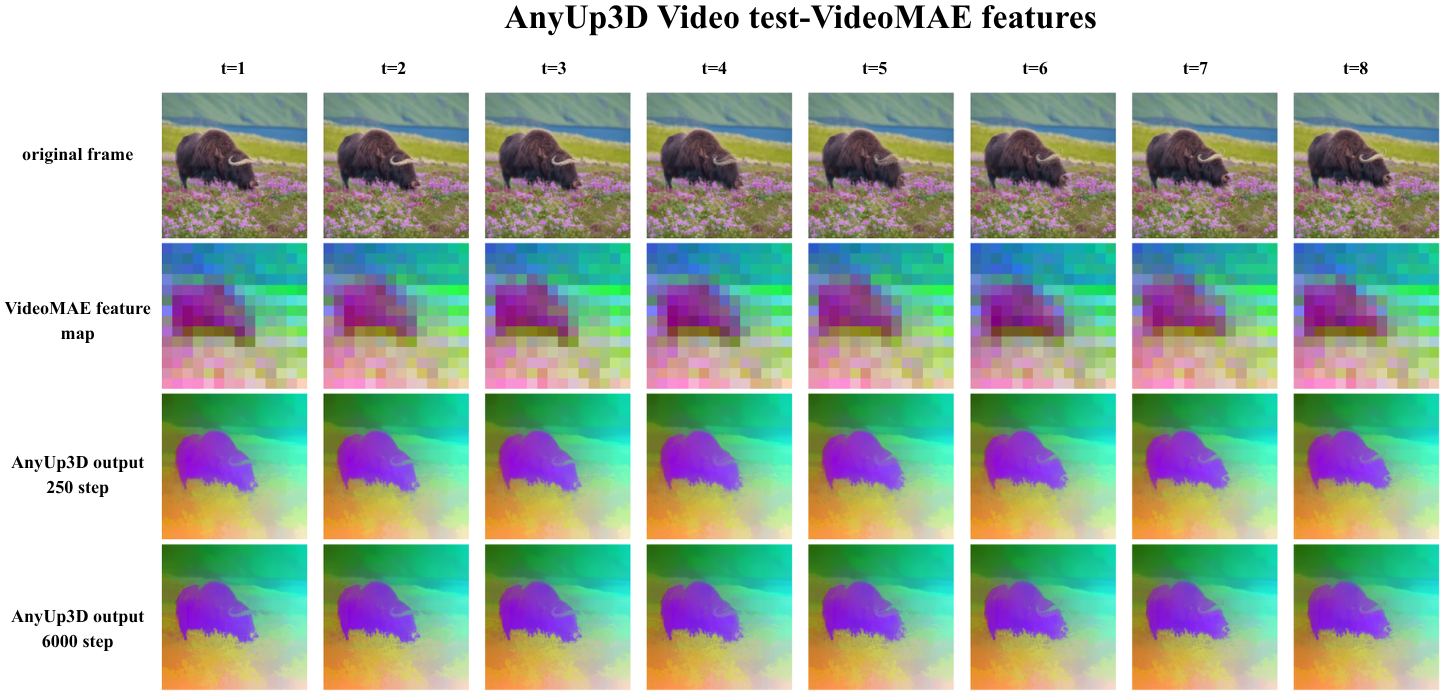
\includegraphics[width=\linewidth]{Figures/AnyUP3D vs VideoMAE feature.jpg}
    \caption{%
        Qualitative comparison of VideoMAE input features and AnyUp3D outputs across training.
        \textbf{Top:} original video frames.
        \textbf{Second row:} PCA visualization of the low-resolution VideoMAE feature maps.
        \textbf{Third row:} AnyUp3D output at step~250.
        \textbf{Bottom:} AnyUp3D output at step~6{,}000, showing clearer object boundaries and more spatially coherent high-resolution features.
    }
    \label{fig:convergence}
\end{figure}

Figure~\ref{fig:convergence} shows the comparison.
At step~250, the PCA visualization reveals features that are spatially disorganized: colors shift abruptly between adjacent pixels and bear little correspondence to the objects visible in the RGB frames.
This is expected, as the model has had minimal training and the cross-attention weights have not yet learned to align features with the spatial structure of the guide image.

By step~6{,}000, the upsampled features exhibit clear spatial organization.
Object boundaries — such as the outline of the ball and the person's silhouette — are sharply delineated in the PCA space.
The PCA colors remain consistent across frames for the same object, indicating that the model produces temporally stable features in addition to spatially coherent ones.
The background, foreground object, and person are assigned distinct and stable feature clusters throughout the sequence.

This comparison confirms that AnyUp3D learns to exploit the RGB guide for spatially informed upsampling over the course of training, rather than producing a trivial interpolation of the input features.


% ────────────────────────────────────────────
\section{Experiment 2: Temporal Feature Consistency}
\label{sec:temporal}

The central claim of AnyUp3D is that jointly processing the temporal dimension produces more temporally coherent features than applying a 2D upsampler independently to each frame.
This experiment tests that claim directly.

\subsection{Setup}

For each of the 30 video clips in the DAVIS~2017 validation set, we extract VideoMAE features and upsample them using two methods: (1)~2D~AnyUp applied independently to each frame, and (2)~AnyUp3D applied to the full spatiotemporal volume.
We then measure temporal consistency as the mean cosine similarity between the feature maps of adjacent frames.
Concretely, for an output tensor of shape $(1, C, T', H, W)$, we compute:
\begin{equation}
    \text{TemporalSim} = \frac{1}{T'-1} \sum_{t=0}^{T'-2}
    \text{cos}\!\left(\mathbf{q}_t,\, \mathbf{q}_{t+1}\right),
    \label{eq:temporal_sim}
\end{equation}
where $\mathbf{q}_t \in \mathbb{R}^{C \cdot H \cdot W}$ is the flattened feature map at time step~$t$.
Higher values indicate greater temporal stability — that is, features that change smoothly between adjacent frames rather than flickering.

\subsection{Results}

Table~\ref{tab:temporal} reports per-clip cosine similarity for all 30 DAVIS~2017 validation clips.

\begin{table}[t]
\centering
\caption{%
    Temporal feature consistency (adjacent-frame cosine similarity, higher is better) on DAVIS~2017 validation clips.
    AnyUp3D improves consistency on every clip, with a mean improvement of $+0.081$.
}
\label{tab:temporal}
\small
\begin{tabular}{lccc}
\toprule
\textbf{Clip} & \textbf{2D AnyUp} & \textbf{AnyUp3D} & \textbf{$\Delta$} \\
\midrule
bike-packing       & 0.879 & 0.974 & +0.095 \\
blackswan          & 0.917 & 0.971 & +0.054 \\
bmx-trees          & 0.810 & 0.928 & +0.118 \\
breakdance         & 0.875 & 0.978 & +0.103 \\
camel              & 0.902 & 0.973 & +0.071 \\
car-roundabout     & 0.893 & 0.950 & +0.057 \\
car-shadow         & 0.927 & 0.967 & +0.039 \\
cows               & 0.914 & 0.978 & +0.064 \\
dance-twirl        & 0.869 & 0.952 & +0.083 \\
dog                & 0.807 & 0.925 & +0.118 \\
dogs-jump          & 0.916 & 0.975 & +0.059 \\
drift-chicane      & 0.906 & 0.975 & +0.069 \\
drift-straight     & 0.812 & 0.901 & +0.089 \\
goat               & 0.859 & 0.952 & +0.093 \\
gold-fish          & 0.911 & 0.976 & +0.065 \\
horsejump-high     & 0.895 & 0.961 & +0.066 \\
india              & 0.764 & 0.896 & +0.132 \\
judo               & 0.901 & 0.986 & +0.085 \\
kite-surf          & 0.891 & 0.958 & +0.067 \\
lab-coat           & 0.858 & 0.932 & +0.074 \\
libby              & 0.856 & 0.935 & +0.080 \\
loading            & 0.846 & 0.933 & +0.087 \\
mbike-trick        & 0.886 & 0.964 & +0.078 \\
motocross-jump     & 0.681 & 0.805 & +0.124 \\
paragliding-launch & 0.909 & 0.966 & +0.057 \\
parkour            & 0.819 & 0.910 & +0.091 \\
pigs               & 0.908 & 0.976 & +0.067 \\
scooter-black      & 0.867 & 0.924 & +0.057 \\
shooting           & 0.776 & 0.885 & +0.109 \\
soapbox            & 0.826 & 0.908 & +0.083 \\
\midrule
\textbf{Mean $\pm$ Std} & $0.863 \pm 0.055$ & $0.944 \pm 0.038$ & $\mathbf{+0.081}$ \\
\bottomrule
\end{tabular}
\end{table}

AnyUp3D achieves higher temporal consistency than 2D~AnyUp on every single clip in the dataset, with no exceptions.
The mean cosine similarity increases from $0.863$ to $0.944$, an improvement of $+0.081$.
The standard deviation also decreases from $0.055$ to $0.038$, indicating that AnyUp3D produces consistently stable features regardless of the motion characteristics of the input clip.

The largest improvements occur on clips with challenging motion.
\textit{india} ($+0.132$), \textit{motocross-jump} ($+0.124$), \textit{bmx-trees} ($+0.118$), and \textit{dog} ($+0.118$) are among the clips where 2D~AnyUp struggles most (lowest baseline scores), and these are precisely where the temporal modeling of AnyUp3D provides the greatest benefit.
These clips contain either fast camera motion, rapid object displacement, or both — conditions under which frame-independent processing introduces the most inter-frame inconsistency.

Even on clips where the 2D baseline already performs well (e.g., \textit{car-shadow} at $0.927$), AnyUp3D still improves consistency, reaching $0.967$.
This demonstrates that the temporal extension does not merely compensate for difficult cases but provides a consistent benefit across the full range of video content.

% ── FIGURE: PCA comparison ──
\begin{figure}[t]
    \centering
    % [Figure 2: PCA visualization comparing 2D AnyUp vs AnyUp3D
    %  on the same DAVIS clip. Two rows of 8 frames each:
    %  Row 1: 2D AnyUp (frame-independent) — PCA colors flicker
    %          between adjacent frames.
    %  Row 2: AnyUp3D — PCA colors remain stable across time,
    %          with consistent object-to-color mapping.]
    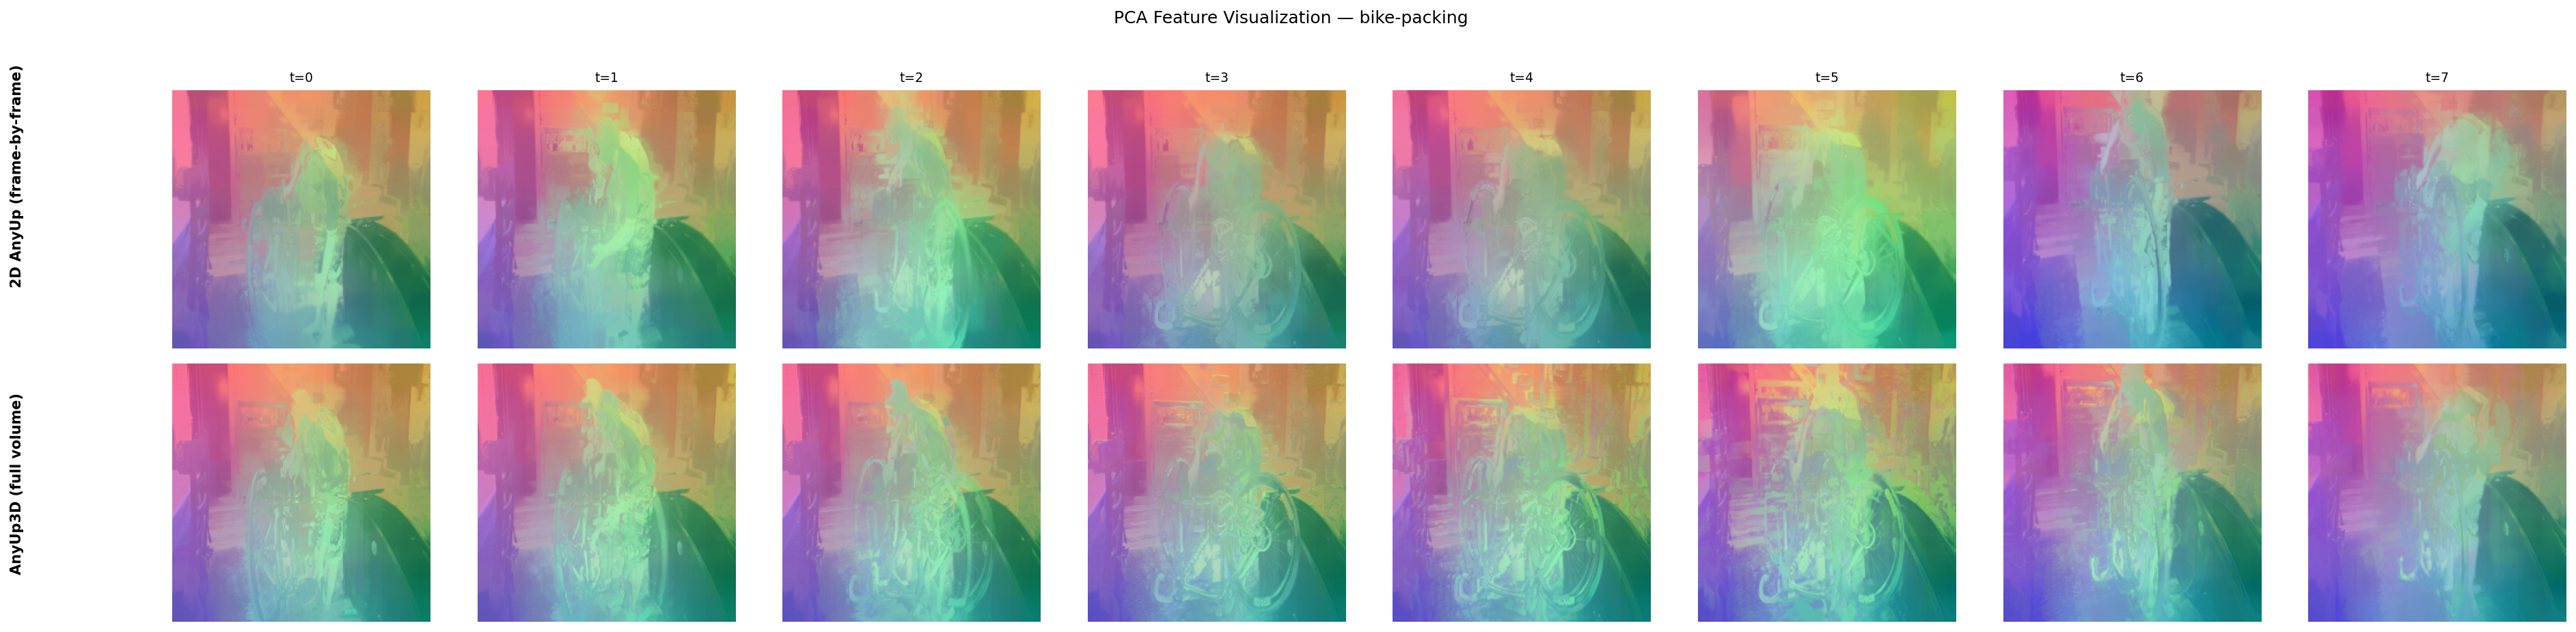
\includegraphics[width=\linewidth]{Figures/pca_bike-packing.png}
    \caption{%
        PCA visualization of upsampled features on a representative DAVIS clip.
        \textbf{Top:} 2D~AnyUp applied frame-independently — PCA colors shift between frames, indicating temporal inconsistency in the feature space.
        \textbf{Bottom:} AnyUp3D — PCA colors remain stable across frames, with consistent object-to-color assignments throughout the sequence.
    }
    \label{fig:pca_comparison}
\end{figure}

Figure~\ref{fig:pca_comparison} provides a qualitative illustration of this effect.
When 2D~AnyUp is applied frame by frame, the PCA colors assigned to the same object can shift noticeably between consecutive frames, even when the object itself barely moves.
With AnyUp3D, the same object maintains a consistent PCA color throughout the sequence, confirming that the model produces a temporally coherent feature space.


% ────────────────────────────────────────────
\section{Experiment 3: Downstream Video Object Segmentation}
\label{sec:jf}

While Experiment~2 measures feature-level consistency, it does not directly assess whether the upsampled features are useful for a downstream task.
This experiment evaluates AnyUp3D features in a practical video object segmentation pipeline using the standard $\mathcal{J}\&\mathcal{F}$ metric.

\subsection{Setup}

We construct a simple segmentation pipeline: VideoMAE extracts spatiotemporal features, the upsampler (either bilinear interpolation or AnyUp3D) produces features at $224 \times 224$ resolution, and a linear segmentation head (a single $1 \times 1$ convolution) predicts per-pixel masks.
The segmentation head is trained identically for both conditions.
We evaluate on all 30 clips of the DAVIS~2017 validation set using the standard $\mathcal{J}\&\mathcal{F}$ score, where $\mathcal{J}$ measures region overlap (Jaccard index) and $\mathcal{F}$ measures contour accuracy.

It is important to note that the absolute $\mathcal{J}\&\mathcal{F}$ scores in this experiment are not directly comparable to dedicated video object segmentation methods (e.g., STM~\cite{stm}, XMem~\cite{xmem}), which typically achieve scores above $0.80$ on DAVIS~2017.
Our pipeline uses VideoMAE features — designed for video understanding, not segmentation — with a minimal linear head and no test-time adaptation.
The purpose of this experiment is not to compete with VOS methods but to measure whether AnyUp3D features carry more useful spatial information than bilinearly upsampled features when used with an identical downstream head.

\subsection{Results}

Table~\ref{tab:jf} reports per-clip $\mathcal{J}\&\mathcal{F}$ scores for a representative subset of 9~clips along with the mean computed over all 30 clips.

\begin{table}[t]
\centering
\caption{%
    Video object segmentation results ($\mathcal{J}\&\mathcal{F}$, higher is better) on DAVIS~2017.
    Per-clip scores shown for a representative subset; the mean is computed over all 30 validation clips.
    AnyUp3D improves the mean $\mathcal{J}\&\mathcal{F}$ by $+0.110$ over bilinear upsampling.
}
\label{tab:jf}
\small
\begin{tabular}{lccc|ccc|cc}
\toprule
 & \multicolumn{3}{c|}{\textbf{Bilinear}} & \multicolumn{3}{c|}{\textbf{AnyUp3D}} & \\
\textbf{Clip} & $\mathcal{J}$ & $\mathcal{F}$ & $\mathcal{J}\&\mathcal{F}$ & $\mathcal{J}$ & $\mathcal{F}$ & $\mathcal{J}\&\mathcal{F}$ & $\Delta$ \\
\midrule
bike-packing    & 0.404 & 0.092 & 0.248 & 0.436 & 0.152 & 0.294 & +0.046 \\
blackswan       & 0.707 & 0.128 & 0.418 & 0.769 & 0.206 & 0.487 & +0.070 \\
bmx-trees       & 0.259 & 0.118 & 0.189 & 0.162 & 0.100 & 0.131 & $-$0.058 \\
camel           & 0.668 & 0.106 & 0.387 & 0.742 & 0.245 & 0.494 & +0.107 \\
car-roundabout  & 0.827 & 0.131 & 0.479 & 0.843 & 0.197 & 0.520 & +0.040 \\
car-shadow      & 0.667 & 0.094 & 0.380 & 0.420 & 0.093 & 0.257 & $-$0.124 \\
cows            & 0.714 & 0.114 & 0.414 & 0.715 & 0.172 & 0.444 & +0.029 \\
dance-twirl     & 0.487 & 0.094 & 0.290 & 0.476 & 0.152 & 0.314 & +0.024 \\
dog             & 0.607 & 0.112 & 0.359 & 0.518 & 0.110 & 0.314 & $-$0.045 \\
\midrule
\textbf{Mean (all 30)} & 0.416 & 0.087 & 0.251 & 0.565 & 0.158 & 0.362 & $\mathbf{+0.110}$ \\
\bottomrule
\end{tabular}
\end{table}

Across all 30 DAVIS clips, AnyUp3D achieves a mean $\mathcal{J}\&\mathcal{F}$ of $0.362$ compared to $0.251$ for bilinear upsampling, an improvement of $+0.110$.
Both components improve: the region overlap $\mathcal{J}$ increases from $0.416$ to $0.565$ ($+0.149$), and the contour accuracy $\mathcal{F}$ increases from $0.087$ to $0.158$ ($+0.071$).
The improvement in $\mathcal{F}$ is particularly relevant: it indicates that AnyUp3D features produce sharper object boundaries than bilinear features, which is a direct consequence of the guided cross-attention mechanism inheriting spatial detail from the RGB guide image.

\subsection{Failure Cases}
\label{sec:failures}

Three of the nine representative clips show a decrease in $\mathcal{J}\&\mathcal{F}$ with AnyUp3D: \textit{car-shadow} ($-0.124$), \textit{bmx-trees} ($-0.058$), and \textit{dog} ($-0.045$).

\textit{Car-shadow} is the most significant regression.
In this clip, the target object is a car accompanied by its shadow on the road surface.
The shadow has low contrast against the background, and the bilinear baseline benefits from the spatial smoothing that blurs the shadow region into a connected mass.
AnyUp3D, by sharpening boundaries, may fragment the shadow into disconnected regions that the linear head fails to unify, resulting in a lower region overlap score.

\textit{Bmx-trees} contains fast, erratic motion of a small object (a cyclist) against a cluttered background.
The RGB-difference gate in the temporal consistency loss likely excluded many frame pairs during training for this type of motion, leaving the model with weaker temporal priors for fast-moving small objects.

\textit{Dog} shows a moderate regression.
The clip features a dog moving against a visually similar background, where the fine-grained boundary sharpening of AnyUp3D may not consistently improve region overlap when the object-background contrast in feature space is inherently low.

These failure cases share a common pattern: AnyUp3D's boundary-sharpening behavior, which improves $\mathcal{F}$ on most clips, can reduce $\mathcal{J}$ when it fragments regions that the linear head cannot recover.
A more expressive segmentation head (e.g., a multi-layer decoder) would likely mitigate this effect, but we deliberately use a linear head to isolate the quality of the features themselves.

% ── FIGURE: Qualitative segmentation comparison ──
\begin{figure}[t]
    \centering
    % [Figure 3: Side-by-side segmentation results for 3-4 clips.
    %  Three columns per clip: Original frame | Bilinear mask overlay
    %  | AnyUp3D mask overlay. Include at least one success case
    %  (e.g., camel or blackswan) and one failure case (e.g., car-shadow).]
    \safeincludegraphics[width=\textwidth]{Figures/segmentation_comparison.png}
    \caption{%
        Qualitative segmentation results on DAVIS~2017 clips.
        Each group shows the original frame, the segmentation mask from bilinear-upsampled features, and the mask from AnyUp3D features.
        AnyUp3D typically produces sharper object boundaries (e.g., \textit{camel}, \textit{blackswan}), but can fragment low-contrast regions (e.g., \textit{car-shadow}).
    }
    \label{fig:segmentation}
\end{figure}


% ────────────────────────────────────────────
\section{Discussion and Limitations}
\label{sec:discussion}

\subsection{Summary of Findings}

The three experiments provide complementary evidence for AnyUp3D's effectiveness.
The training convergence analysis (Experiment~1) confirms that the model learns to exploit the RGB guide for spatially structured upsampling.
The temporal consistency evaluation (Experiment~2) demonstrates that AnyUp3D produces substantially more stable features than frame-independent 2D upsampling, with improvements on all 30 DAVIS clips and a mean cosine similarity increase of $+0.081$.
The downstream segmentation evaluation (Experiment~3) shows that these feature improvements translate into practical task-level gains, with a mean $\mathcal{J}\&\mathcal{F}$ improvement of $+0.110$.

\subsection{Limitations}

Several limitations of this evaluation should be acknowledged.

\paragraph{No spatial-only benchmark.}
The original evaluation plan included a linear probing experiment on a standard image segmentation dataset (e.g., ADE20K) to measure spatial upsampling quality in isolation, using mIoU as the metric.
This experiment was not conducted due to time constraints.
Instead, Experiment~1 provides qualitative evidence of spatial quality through PCA visualization, and Experiment~3 provides indirect quantitative evidence through the $\mathcal{F}$-score improvement.
A dedicated spatial benchmark would strengthen the evaluation by providing a direct, quantitative comparison of spatial feature quality independent of temporal effects.

\paragraph{No ablation study.}
We do not present ablation experiments isolating the contributions of individual design decisions — for instance, the effect of removing the RGB guide, replacing the 3D attention with frame-independent 2D attention, or training without the T-curriculum.
Such ablations would clarify which components of the architecture and training strategy are responsible for the observed improvements.

\paragraph{Single training run.}
All results are reported from a single training run rather than averaged over multiple seeds.
While the temporal consistency results are robust (improvements on all 30 clips suggest the result is not seed-dependent), the $\mathcal{J}\&\mathcal{F}$ scores would benefit from multi-seed evaluation with reported confidence intervals.

\paragraph{Limited training budget.}
The model was trained for 6{,}000 steps, compared to 100{,}000 steps for the original 2D~AnyUp~\cite{anyup}.
The relatively low absolute $\mathcal{J}\&\mathcal{F}$ scores — while substantially above the bilinear baseline — suggest that additional training could further improve feature quality.
This is consistent with the training convergence analysis, which shows clear qualitative improvement between step~250 and step~6{,}000 but does not demonstrate convergence.

\paragraph{Backbone choice.}
VideoMAE was chosen for its native spatiotemporal tokenization, which makes it a natural fit for AnyUp3D.
However, VideoMAE features are optimized for video classification, not for dense prediction tasks.
The original evaluation plan specified Video Swin Transformer as the backbone, which produces features more suitable for pixel-level tasks.
The results reported here should be understood as a lower bound on what AnyUp3D can achieve with a backbone better aligned to dense prediction.

\paragraph{Absolute $\mathcal{J}\&\mathcal{F}$ scores.}
The mean $\mathcal{J}\&\mathcal{F}$ scores ($0.251$ for bilinear, $0.362$ for AnyUp3D) are well below the scores achieved by dedicated video object segmentation methods.
This is expected: AnyUp3D is a feature upsampler, not a segmentation model, and the evaluation pipeline uses a minimal linear head with no test-time adaptation.
The relevant comparison is the relative improvement over the bilinear baseline ($+0.110$), not the absolute score level.